\documentclass{seminar}

% From Doc.
\usepackage{amssymb,amsmath}
%\usepackage{ulem}
\usepackage{semlcmss}
%\usepackage{scicomp}
\usepackage{epsfig}
\usepackage{framed}
\usepackage[T1]{fontenc}
\usepackage{multirow}
\usepackage{bm}

% From me
\usepackage{multicol}
\usepackage{ dsfont }


\def\lfoot{Portland State Applied and Computational Math Group} 
\def\rfoot{Michigan Tech University,  Oct. 4 2019}



\begin{document} 
\pagestyle{headings}
%\slidepagestyle{mypagestyle}
\centerslidesfalse

\begin{slide} %%% Title
\begin{center}
Jim's yucky talk \\
wowee
\end{center}
\end{slide} %%% Title




\begin{slide} %%% 1
\large This talk is based on...\small
\begin{center}
	
\includegraphics[scale=0.2]{./PNG/llogo}\\
	%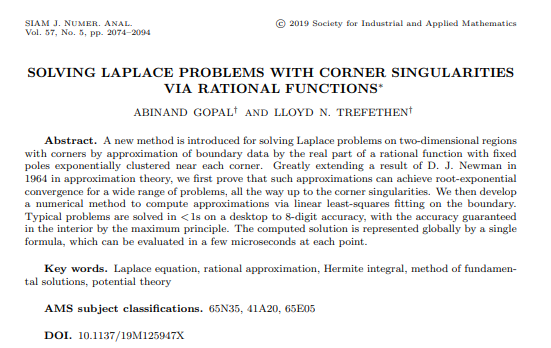
\includegraphics[scale=0.5]{./PNG/paper_abstract}
	\small
	\emph{Solving Laplace Problems with Corner Singularities via Rational Functions}
\end{center}

\begin{itemize}
	\item ...A paper written by Gopal and Trefethen, published in SIAM Journal on Numerical Analysis September 2019
	\item The Lightning Laplace code, based on the paper, yields accurate approximations quickly (on nice problems)
	\item https://epubs.siam.org/doi/pdf/10.1137/19M125947X
	\item https://people.maths.ox.ac.uk/trefethen/lightning.html
\end{itemize}
\end{slide} %%% 1




\begin{slide} %%% 2a
\large Here's the problem\\

\small
We wish to find a (real) function $u$ over a domain $\Omega$ (the complex 2-D plane) which satisfies
\begin{align*}
\Delta u(z)=0, \quad z\in \Omega &&
u(z)=h(z), \quad z\in \Gamma .
\end{align*}
In particular, we want to be able to handle a domain with sharp corners, curves etc. 

We will find $r$, and approximation of $u$ ($u\approx\mathrm{Re}[r]$).
\begin{align*}
r(z)= \sum_{j=1}^{N_1} \frac{a_j}{z-z_j} + \sum_{j=0}^{N_2} b_j (z-z_*)^j
\end{align*}
\end{slide} %%% 2a

\begin{slide} %%% 2b
\large Here's the problem\\

\small
We wish to find a (real) function $u$ over a domain $\Omega$ (the complex 2-D plane) which satisfies
\begin{align*}
\Delta u(z)=0, \quad z\in \Omega &&
u(z)=h(z), \quad z\in \Gamma .
\end{align*}
In particular, we want to be able to handle a domain with sharp corners, curves etc. 

We will find $r$, and approximation of $u$ ($u\approx\mathrm{Re}[r]$).
\begin{align*}
r(z)= \sum_{j=1}^{N_1} \frac{a_j}{z-z_j} + \sum_{j=0}^{N_2} b_j (z-z_*)^j
\end{align*}
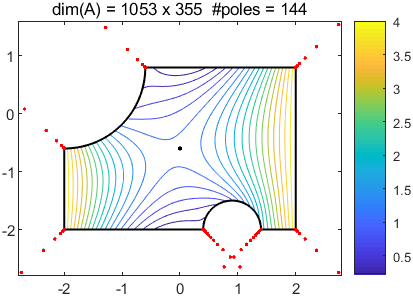
\includegraphics[scale=.45]{./PNG/Howell_1994} $\quad$
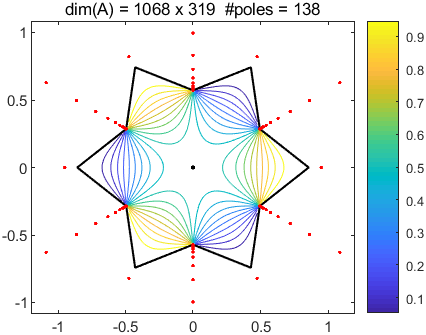
\includegraphics[scale=.4]{./PNG/snowflake}  $\quad$
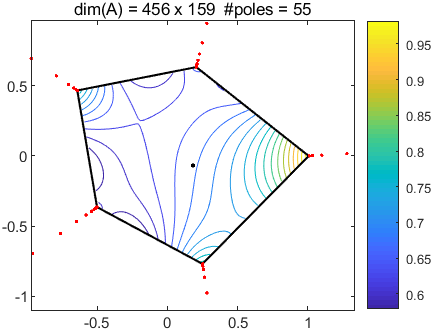
\includegraphics[scale=.4]{./PNG/randpoly1}
\end{slide} %%% 2b




\begin{slide} %%% 3
\large Why this problem?\\

\small
\begin{itemize}
	\item Problems involving the Laplace operator $\Delta={\nabla}^2$ frequently appear in physical equations:
	\begin{itemize}
		\item Heat Equation
		$\alpha {\nabla}^2 u={\partial}_t u$
		\item Schrodinger Equation
		$\left[ \frac{-{\hbar}^2}{2m}{\nabla}^2 + V \right]\Psi=i \hbar \, \partial_t \Psi$
		\item Wave Equation
		$c^2 {\nabla}^2 u={\partial}_t^2 u$
		\item And more...
	\end{itemize}
	\item Functions which satisfy Laplace's Equation have very nice properties, and are called harmonic.
	
\end{itemize}
\end{slide} %%% 3




\begin{slide} %%% 4a
\large Some nice properties of functions of interest \\

\small
\begin{itemize}
	\item The real and imaginary parts of a holomorphic (and thus also an analytic) function $f=u+iv$ are harmonic;
	\item $f$ is also smooth (infinitely differentiable); by extension this applies to $u$ and $v$ as well.
	\item Maximum Principle: a harmonic function on a compact domain attains a max. (and min.) on the boundary.
\end{itemize}
\end{slide} %%% 4a

\begin{slide} %%% 4b
\large Some nice properties of functions of interest \\

\small
\begin{itemize}
	\item The real and imaginary parts of a holomorphic (and thus also an analytic) function $f=u+iv$ are harmonic;
	\item $f$ is also smooth (infinitely differentiable); by extension this applies to $u$ and $v$ as well.
	\item Maximum Principle: a harmonic function on a compact domain attains a max. (and min.) on the boundary.
\end{itemize}

On a simply connected domain we can construct a holomorphic function from a harmonic one: given $u$, define $g=u-iu$. The theory will work with harmonic functions, which will trickle down to our problem.

If $r$ approximates $f$, having real part $u$, the worst we'll do over the whole domain in approximating $u$ is $||u(z)-\mathrm{Re}[r(z)]||$, $z \in \Gamma$.
\end{slide} %%% 4b




\begin{slide} %%% 5
\large Back to the problem \\
\small
\begin{align*}
r(z) = \underbrace{\sum_{j=1}^{N_1} \frac{a_j}{z-z_j}}_\text{"Newman"} + \underbrace{\sum_{j=0}^{N_2} b_j (z-z_*)^j}_\text{"Runge"}
\end{align*}

\begin{itemize}
	\item Using the scheme in the paper, we can have root exponentially good approximations for $u$. The task at hand is finding the coefficients $a_j$, $b_j$.
	\begin{align*}
	||f-r_n||_\Omega = O(e^{-C\sqrt{n}})
	\end{align*}
	\item The theorems in the paper are based on interpolation, showing existence.
	\item In the code, the problem is solved via a least squares approach using QR factorization. Code is written in MATLAB.
\end{itemize}
\end{slide} %%% 5




\begin{slide} %%% 6a
\large Describing $r$ 
\small
\begin{align*}
r(z)= \sum_{j=1}^{N_1} \frac{a_j}{z-z_j} + \sum_{j=0}^{N_2} b_j (z-z_*)^j
\end{align*}
The Newman Part: built to handle corners.

\begin{multicols}{2}
\begin{itemize}
	\item The terms $z_j$ are poles, exponentially clustered near a corner on the exterior of $\Omega$ (works for spacing scaled at least $O(n^{-1/2})$).
	\item "Rational functions are more powerful than polynomials for approximating functions near singularities..."\footnote{Lloyd N. Trefethen. 2013. Approximation theory and approximation practice, Society for Industrial and Applied Mathematics.}
\end{itemize}
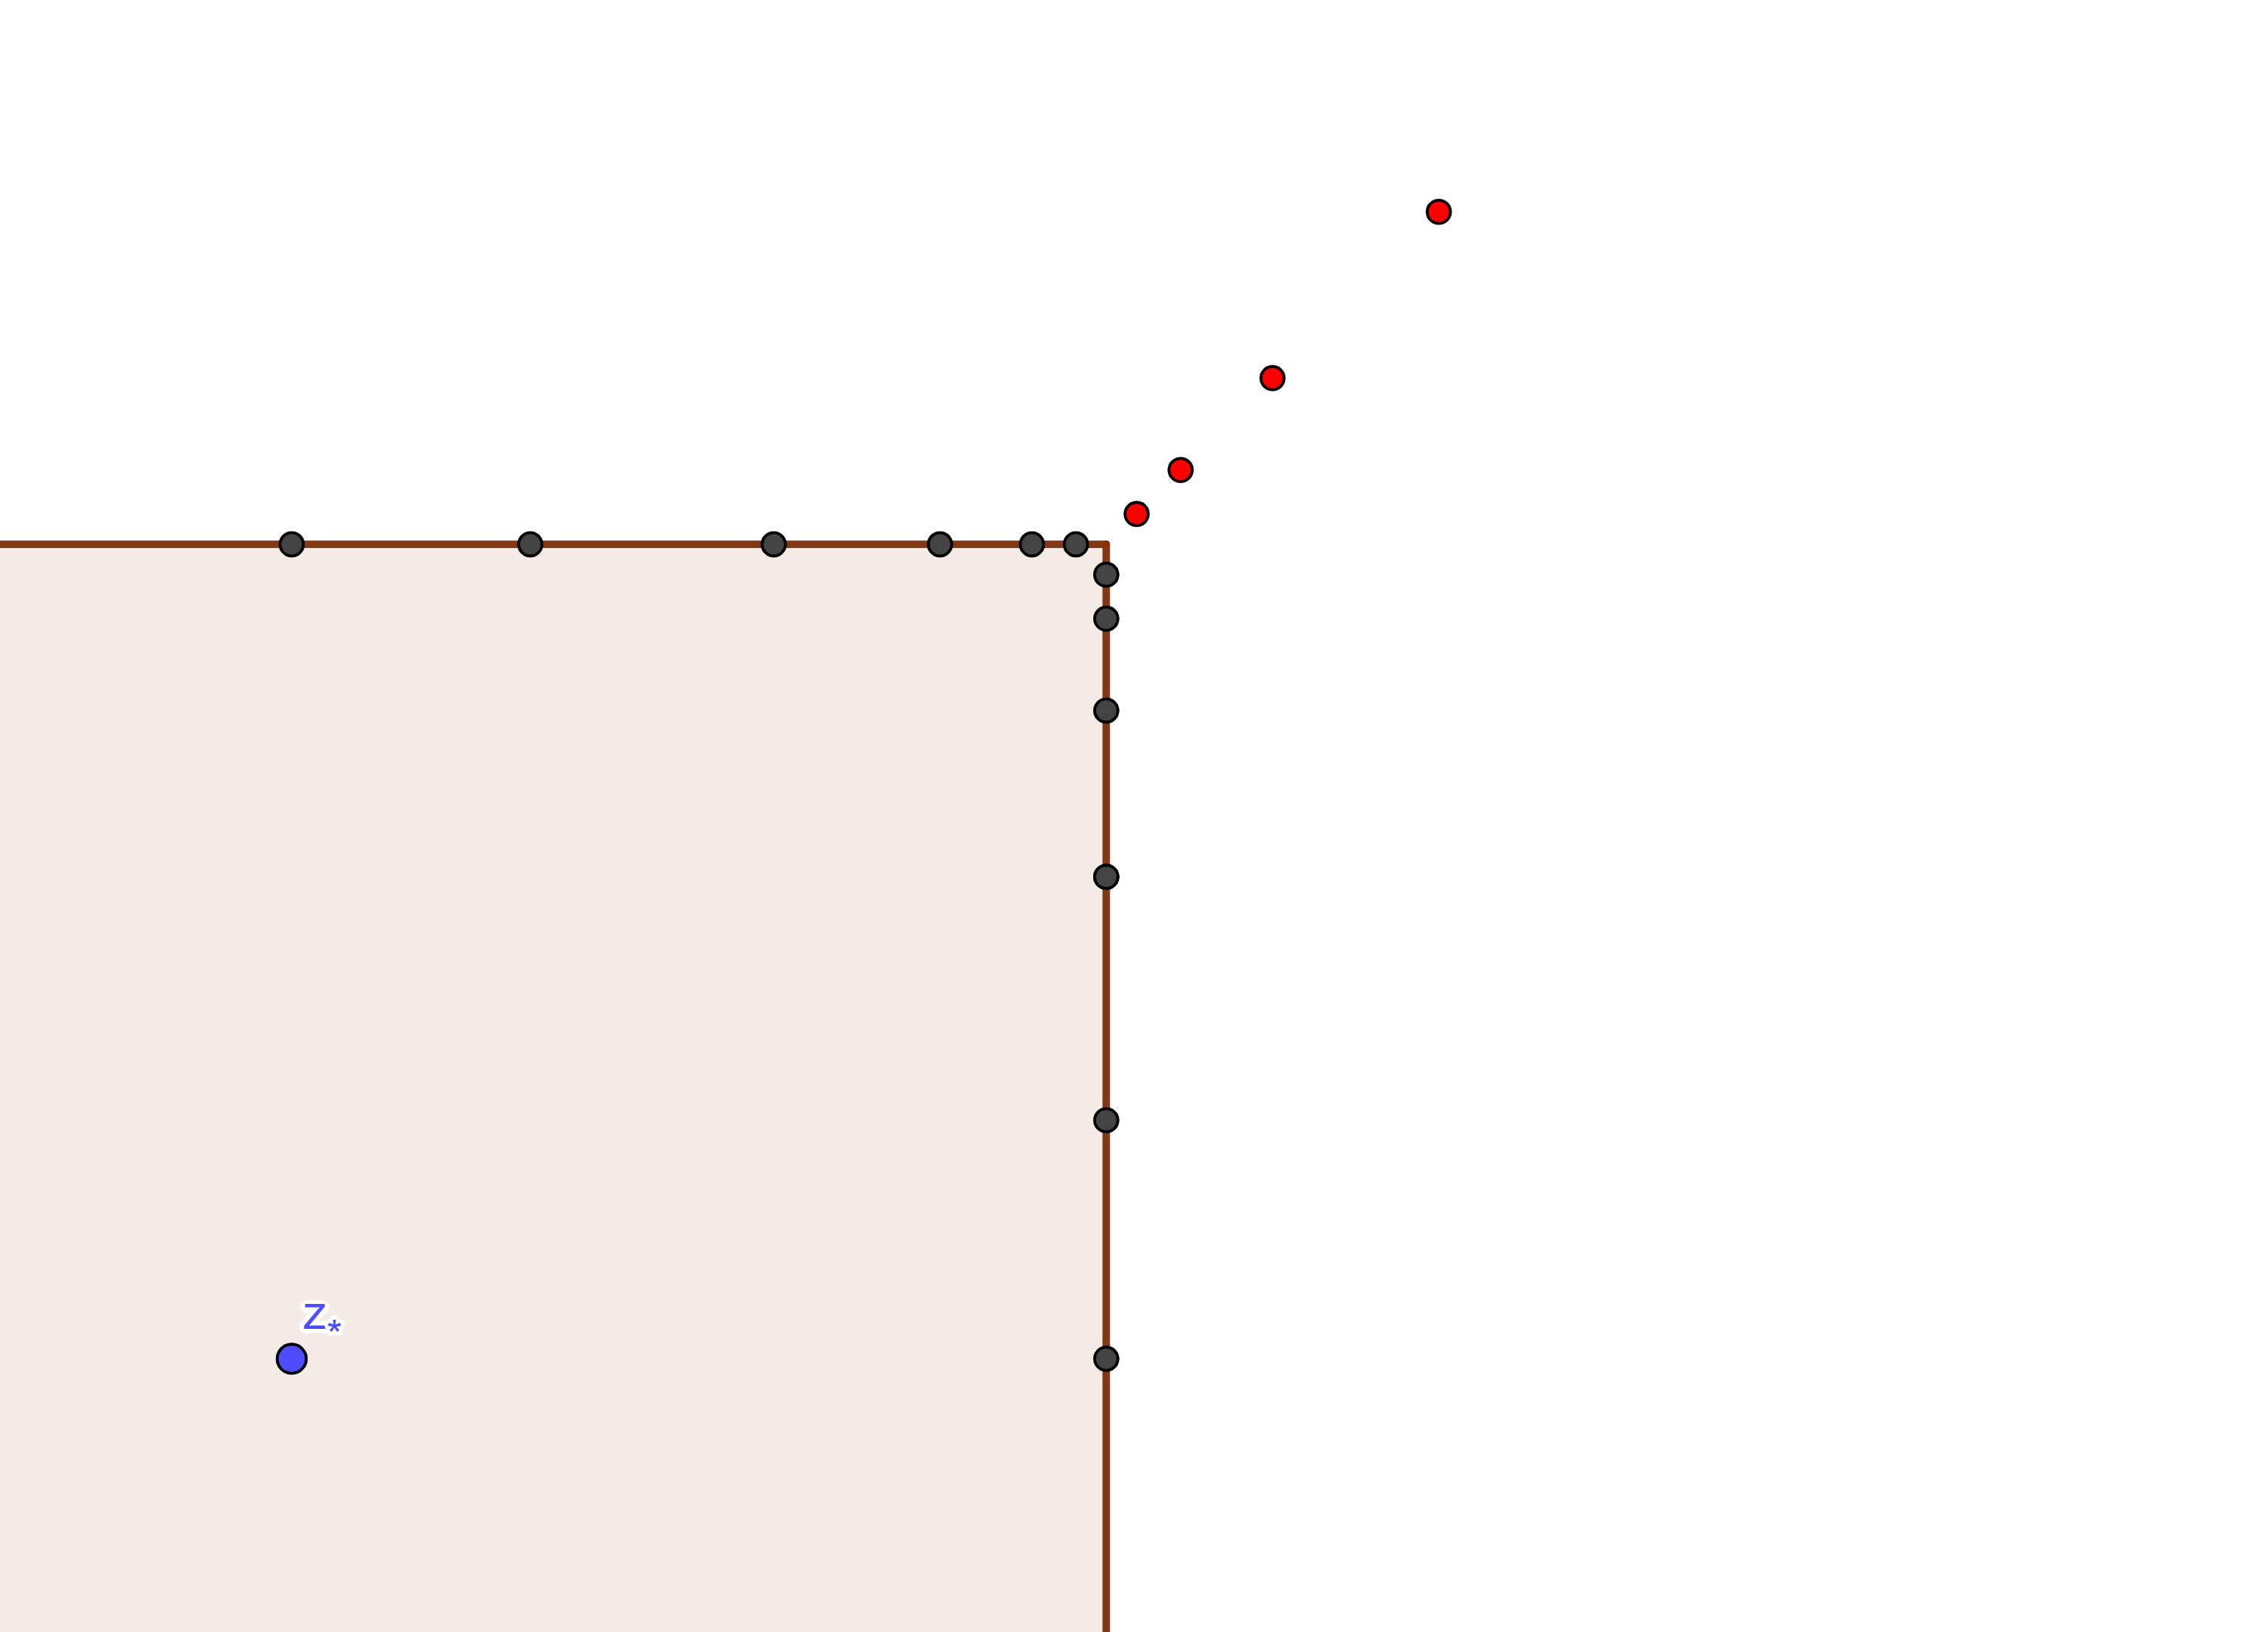
\includegraphics[scale=4]{./PNG/corner_nodes_illust}
\end{multicols}
\end{slide} %%% 6a

\begin{slide} %%% 6b
\large Describing $r$
\small
\begin{align*}
r(z)= \sum_{j=1}^{N_1} \frac{a_j}{z-z_j} + \sum_{j=0}^{N_2} b_j (z-z_*)^j
\end{align*}
The Runge part: built to handle the interior.
\begin{multicols}{2}
\begin{itemize}
	\item The term $z_*$ is an expansion point, near the middle of $\Omega$.
	\item Polynomials can approximate root exponentially well on a nice domain (going back to Runge).
\end{itemize}
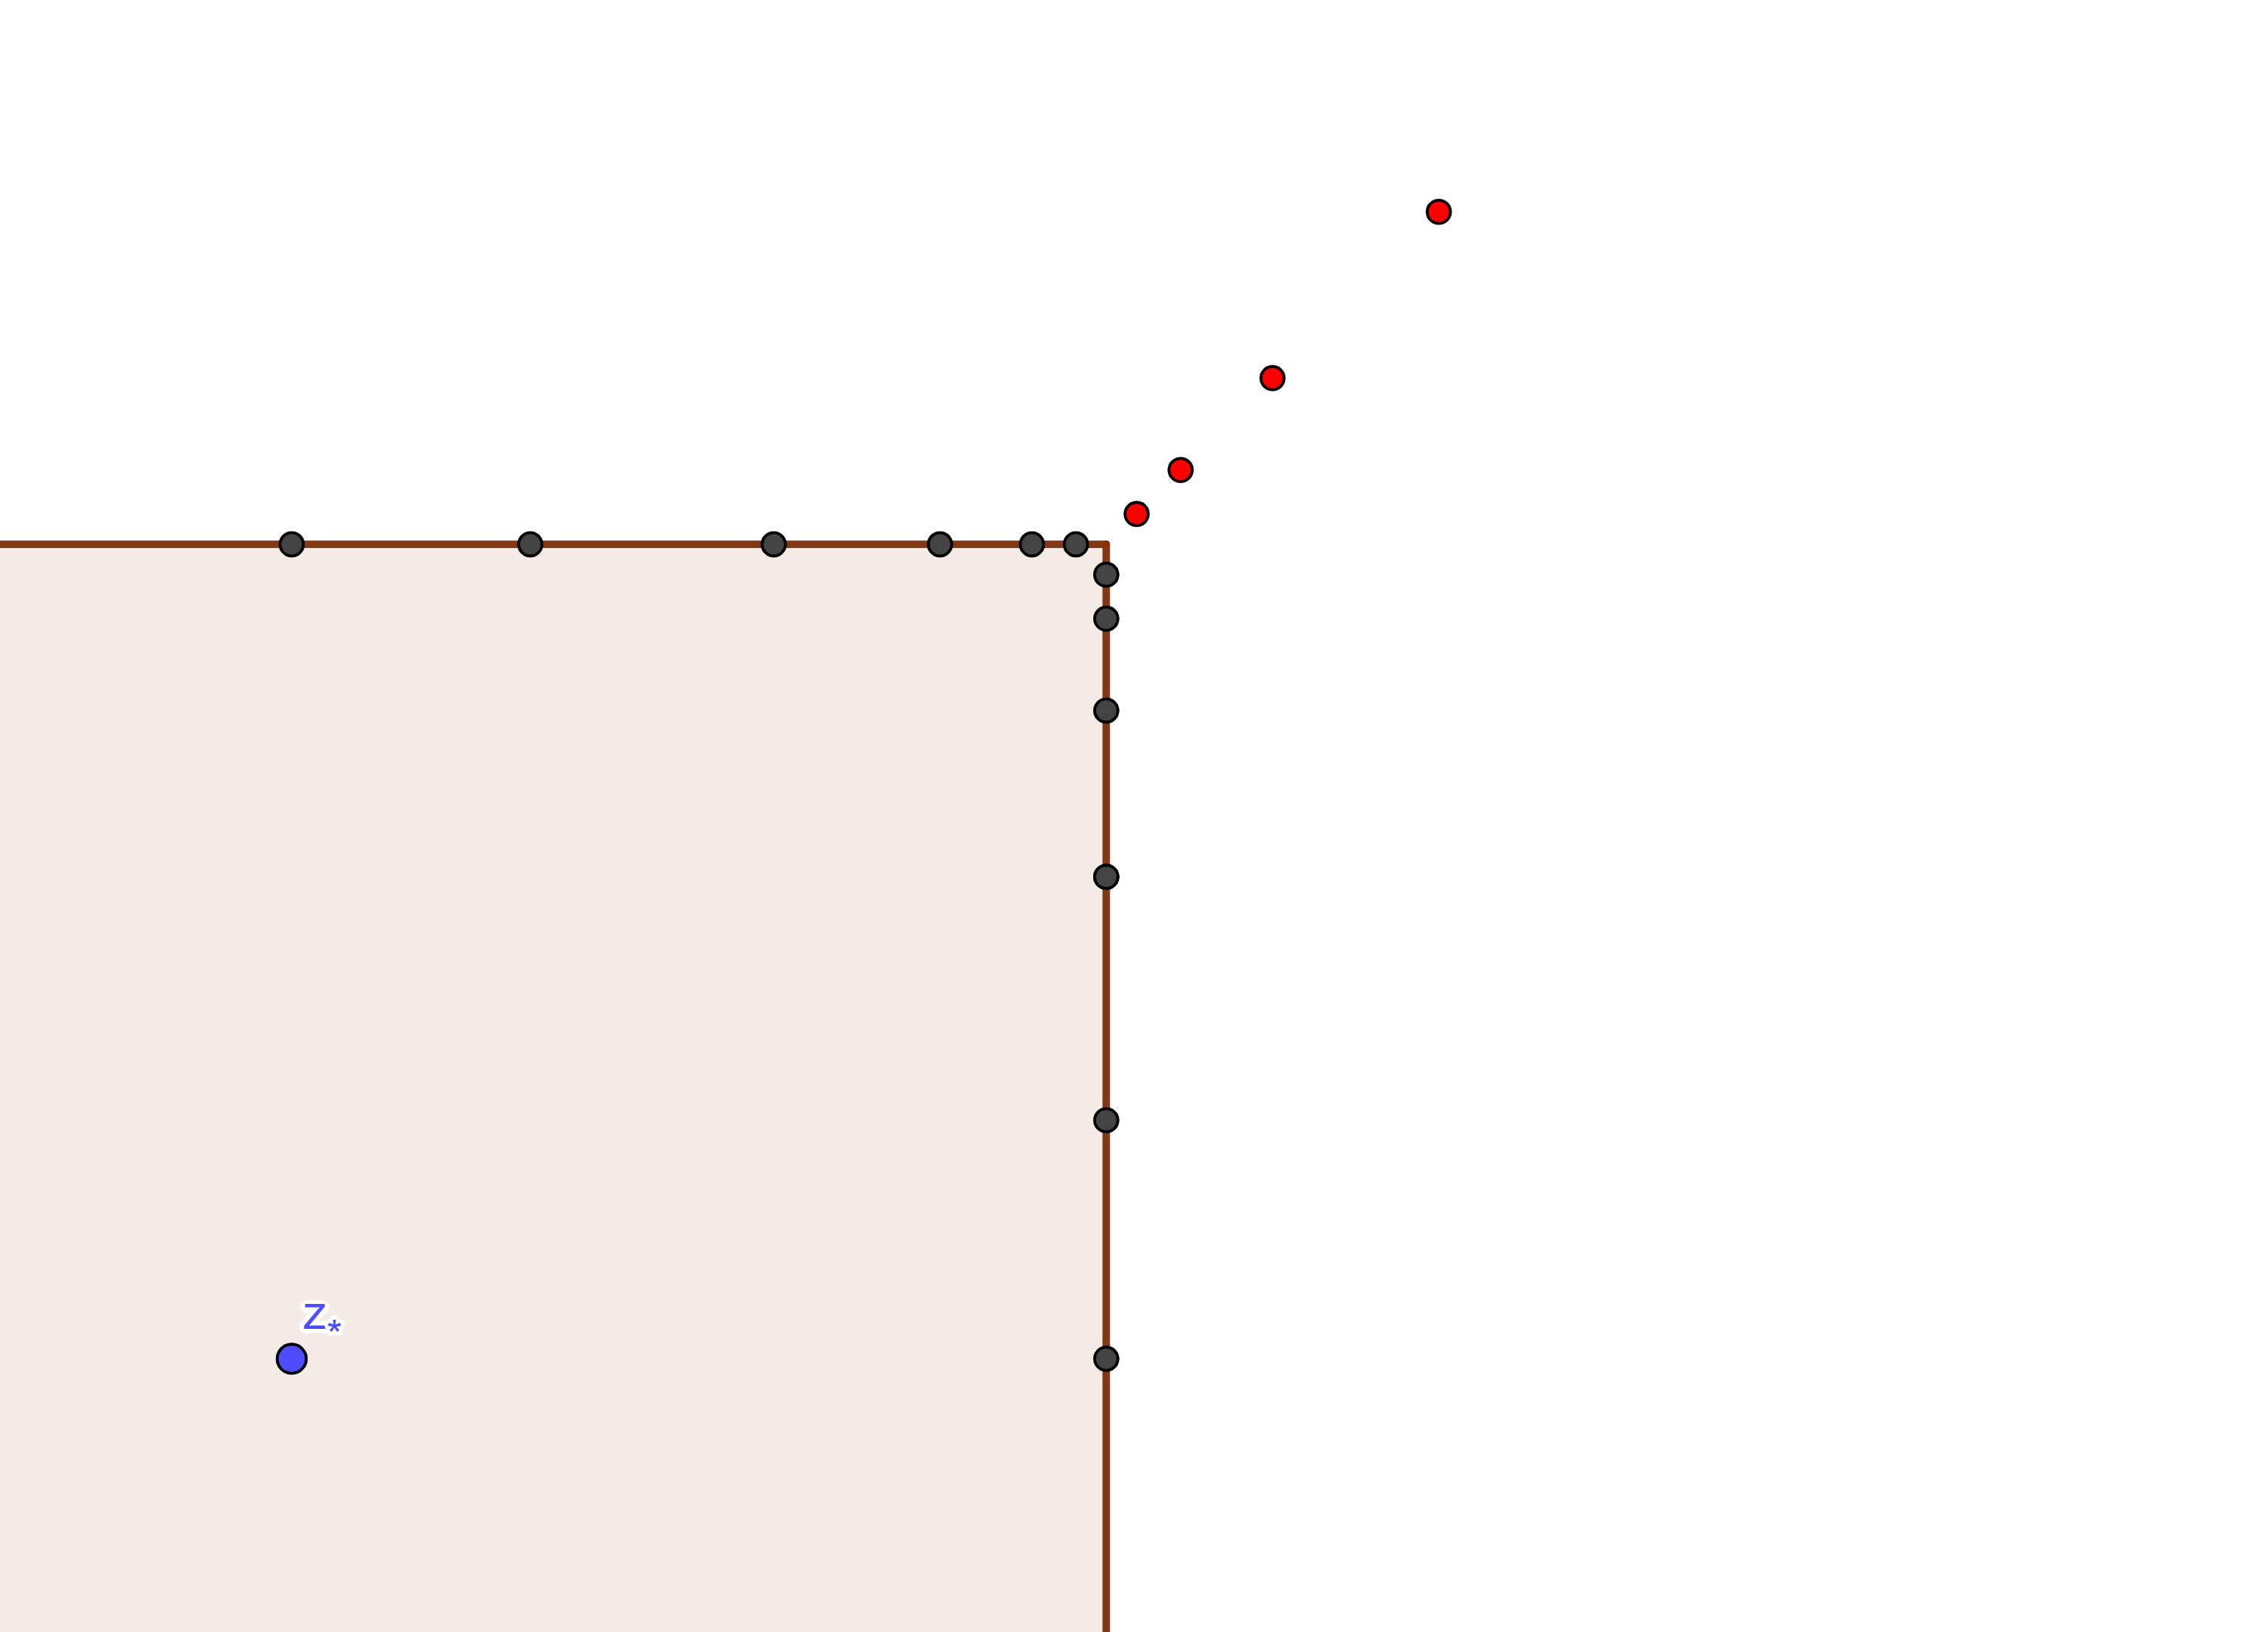
\includegraphics[scale=4]{./PNG/corner_nodes_illust}
\end{multicols}
\end{slide} %%% 6b




\begin{slide} %%% 7a
\large The function $r$ is harmonic 
\small
\begin{align*}
r(z)= \sum_{j=1}^{N_1} \frac{a_j}{z-z_j} + \sum_{j=0}^{N_2} b_j (z-z_*)^j
\end{align*}
To prove $r$ is harmonic, consider $f(z)=1/z$ and $g(z)=z^k$.
The function $f$ can be decomposed as $f=u+iv$, where
\begin{align*}
u(x,y)=\frac{x}{x^2+y^2} &&
v(x,y)=\frac{-y}{x^2+y^2}.
\end{align*}
Taking derivatives will show that $u$ and $v$ satisfy the Cauchy-Riemann equations, ${\partial}_x u={\partial}_y v$, ${\partial}_y u=-{\partial}_x v$.
\end{slide} %%% 7a

\begin{slide} %%% 7b
\large The function $r$ is harmonic 
\small
\begin{align*}
r(z)= \sum_{j=1}^{N_1} \frac{a_j}{z-z_j} + \sum_{j=0}^{N_2} b_j (z-z_*)^j
\end{align*}
To prove $r$ is harmonic, consider $f(z)=1/z$ and $g(z)=z^k$.
The function $f$ can be decomposed as $f=u+iv$, where
\begin{align*}
u(x,y)=\frac{x}{x^2+y^2} &&
v(x,y)=\frac{-y}{x^2+y^2}.
\end{align*}
Taking derivatives will show that $u$ and $v$ satisfy the Cauchy-Riemann equations, ${\partial}_x u={\partial}_y v$, ${\partial}_y u=-{\partial}_x v$, meaning $f$ is (holomorphic, and thus) harmonic.

Writing $g$ in polar form, then in terms of sines and cosines is enough to see $g$ is harmonic:
\begin{align*}
g(z)=\rho e^{i k \theta} = \rho [\cos{(k\theta)} + i \sin{(k\theta)}] .
\end{align*}
Adding these templates, applying translations and scaling as necessary give us our result.
\end{slide} %%% 7b




\begin{slide} %%% 8
\large An important lemma \\

\small
Hermite integral formula for rational interpolation.

Let $\Omega$ be a simply connected domain in $\mathds{C}$ bounded by a closed curve $\Gamma$, and let $f$ be analytic in that domain and extend continuously to the boundary. Let interpolation points ${\alpha}_0, \ldots ,{\alpha}_{n-1} \in \Omega$ and poles ${\beta}_0, \ldots ,{\beta}_{n-1}$ anywhere in the complex plane be given. Let $r$ be the unique type $(n-1,n)$ rational function with simple poles at $\{{\beta}_j\}$ that interpolate $f$ at $\{{\alpha}_j\}$. Then for any $z \in \Omega$,
\begin{align*}
f(z)-r(z)=\frac{1}{2 \pi i} \int_{\Gamma} \frac{\phi (z)}{\phi (t)} \frac{f(t)}{t-z}dt, \\
\phi (z) = \left. \prod_{j=0}^{n-1}(z-{\alpha}_j) \middle/ \prod_{j=0}^{n-1}(z-{\beta}_j). \right.
\end{align*}
\end{slide} %%% 8




\begin{slide} %%% 9
\large First Theorem \\

\small
Let $f$ be a bounded analytic function in the slit disk $A_\pi$ that satisfies $f(z)=O(|z|^\delta)$ as $z \to 0$ for some $\delta > 0$, and let $\theta \in (0,\pi /2)$ be fixed. Then for some $0< \rho < 1$ depending on $\theta$ but not on $f$, there exist type $(n-1,n)$ rational functions $\{r_n\}$, $1 \leq n < \infty$, such that
	\begin{align*}
	||f-r_n||_\Omega = O(e^{-C \sqrt{n}})
	\end{align*}
as $n \to \infty $ for some $C>0$, where $\Omega = \rho A_\theta$. Moreover, each $r_n$ can be taken to have simple poles only at
	\begin{align*}
	\beta_j = -e^{-\sigma j/\sqrt{n}}, \enspace 0\leq j \leq n-1,
	\end{align*}
where $\sigma >0$ is arbitrary.
\end{slide} %%% 9




\begin{slide} %%% 10
\begin{center}
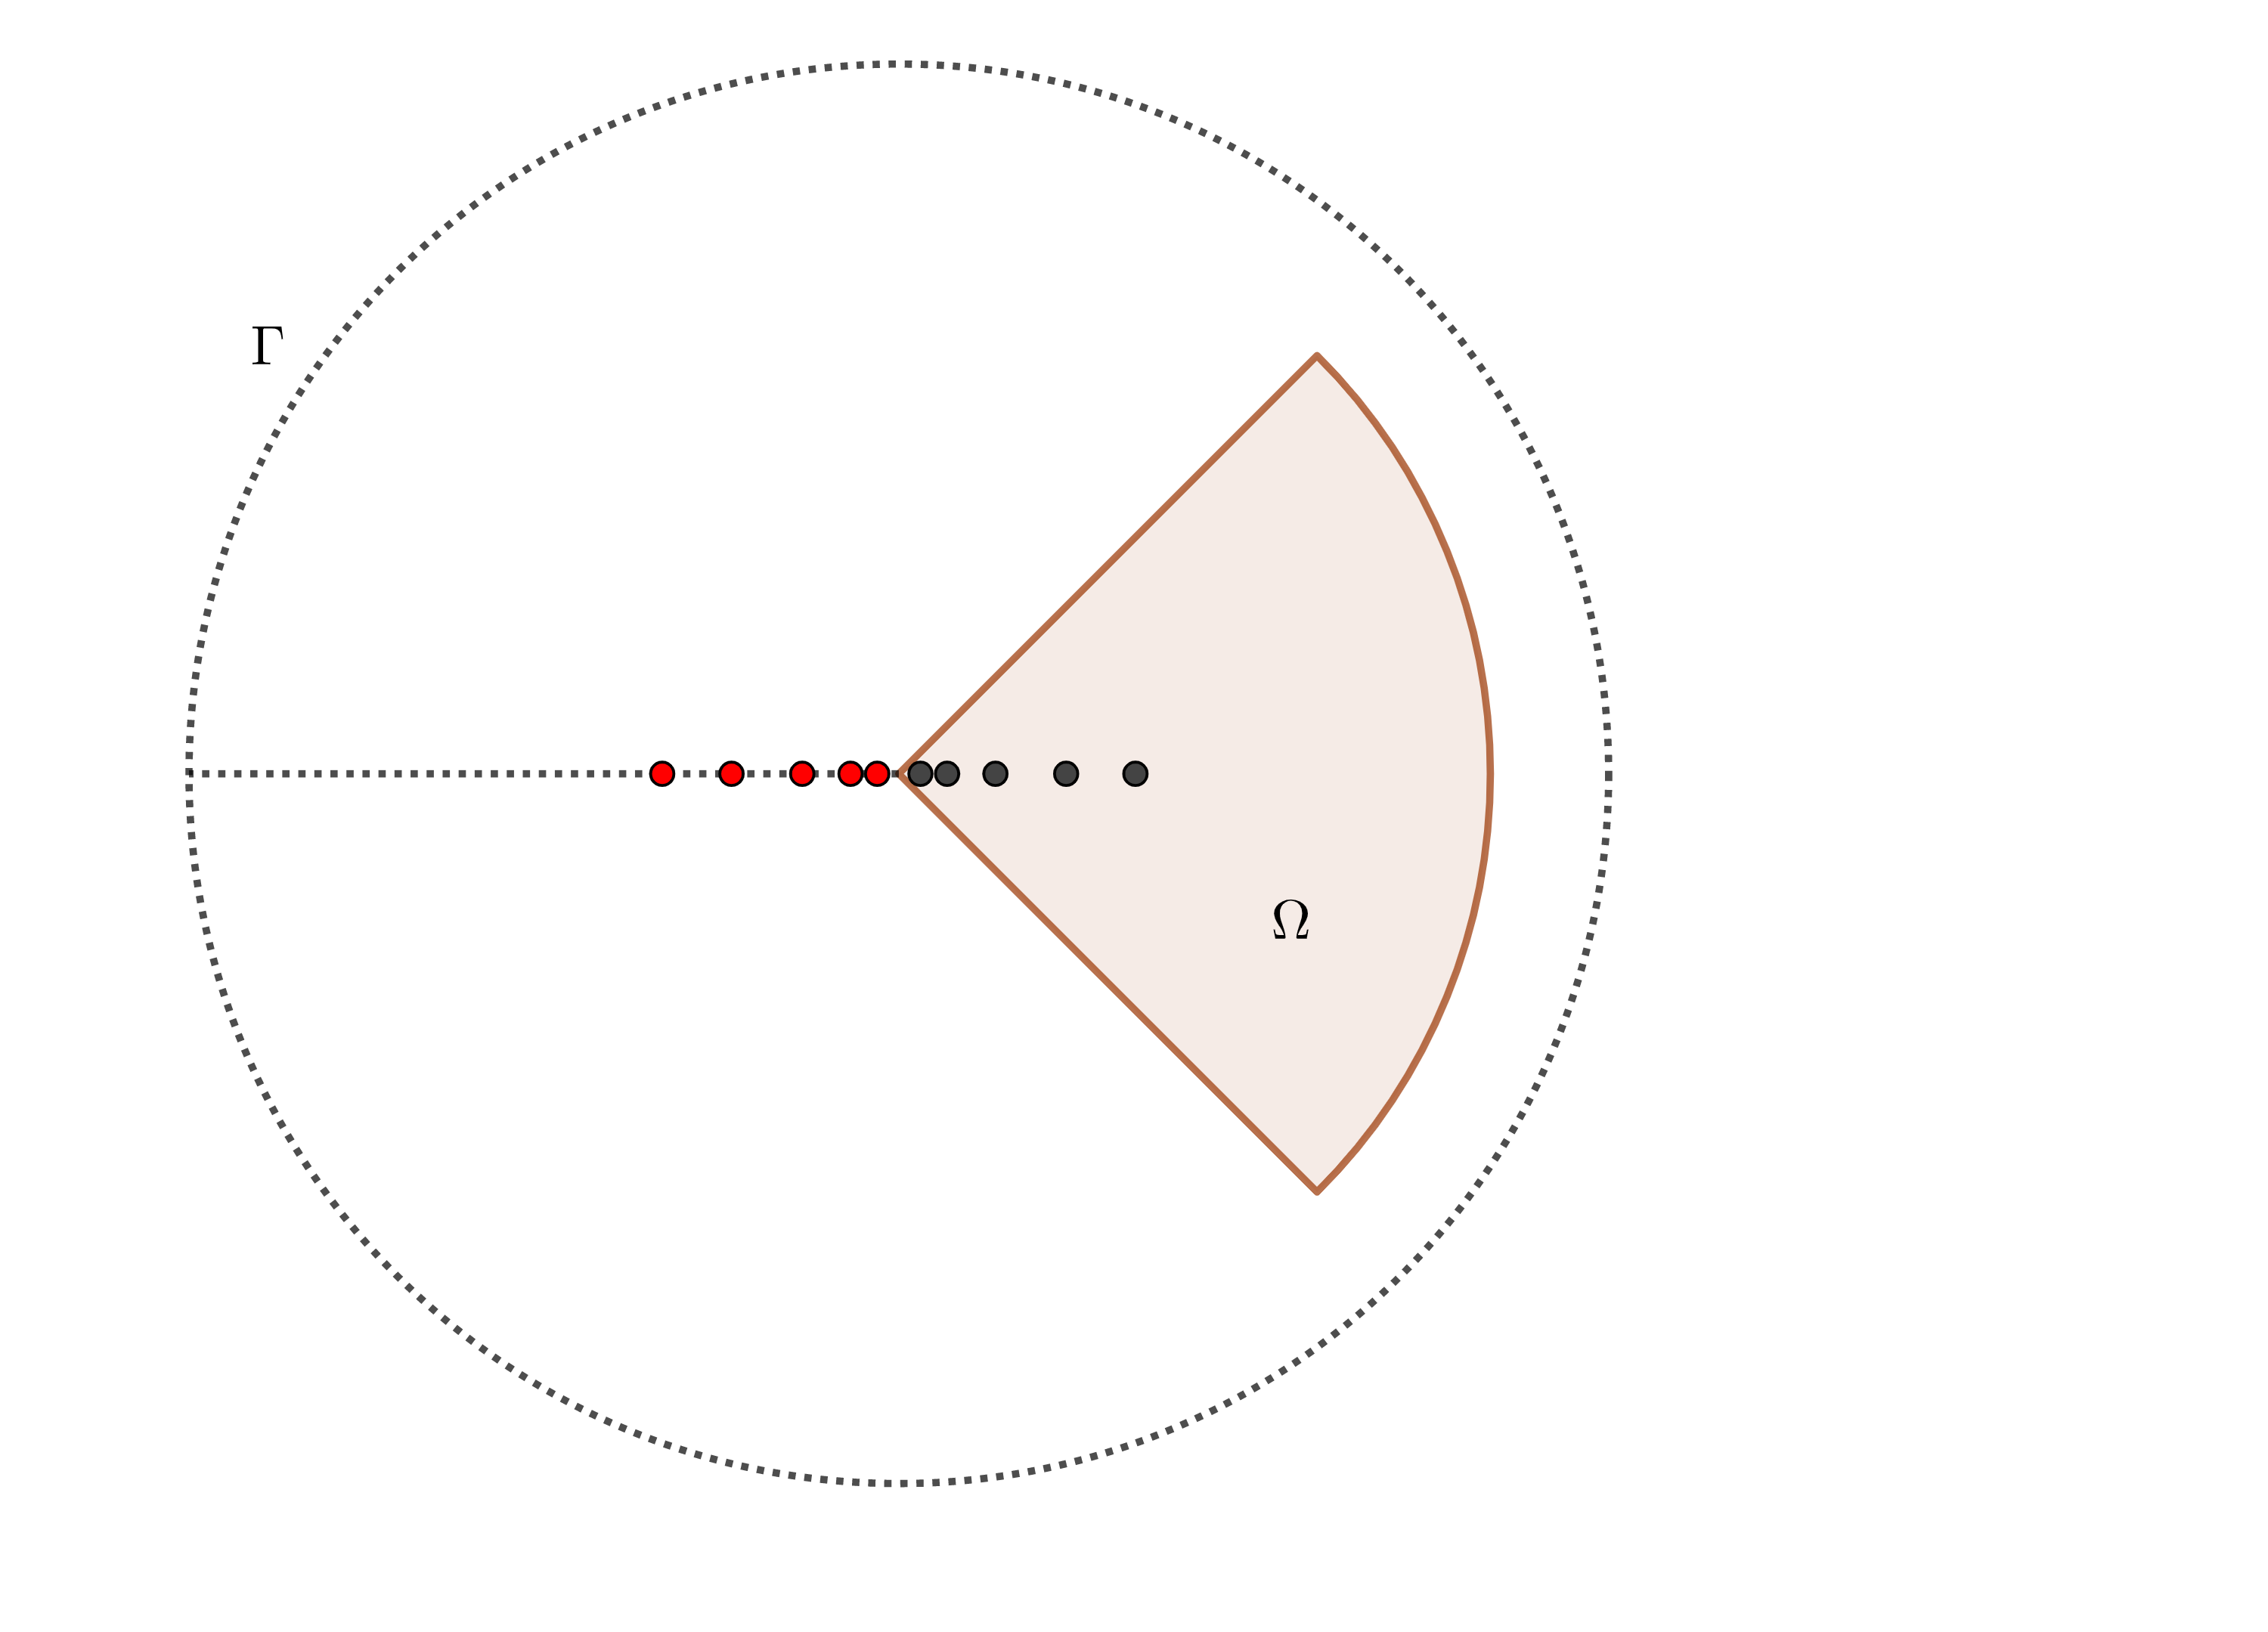
\includegraphics[scale=0.8]{./PNG/A_theta_illust}
\end{center}

\begin{align*}
A_\theta=\{z \in \mathds{C} : |z|<1,\enspace |\mathrm{arg}(z)|<\theta \} &&
\Omega = \rho A_\theta
\end{align*}
\end{slide} %%% 10




\begin{slide} %%% 11
\large Second Theorem \\

\small
Let $\Omega$ be a convex polygon with corners $w_1 , \ldots , w_m$, and let $f$ be an analytic function in $\Omega$ that is analytic on the interior of each side segment and can be analytically continued to a disk near each $w_k$ with a slit along the exterior bisector there. Assume $f$ satisfies $f(z)-f(w_k)=O(|z-w_k|^\delta)$ as $z \to w_k$ for each $k$ for some $\delta >0$. There exist degree $n$ rational functions $\{r_n\},\, 1 \leq n < \infty$ such that
	\begin{align*}
	||f-r_n||_\Omega=O(e^{-C\sqrt{n}})
	\end{align*}
as $n\to \infty$ for some $C>0$. Moreover, each $r_n$ can be taken to have finite poles only at points exponentially clustered along the exterior bisectors at the corners, with arbitrary clustering parameter $\sigma$, as long as the number of poles near each $w_k$ grows at least in proportion to $n$ as $n\to \infty$.
\end{slide} %%% 11




\begin{slide} %%% 12
\large Second Theorem: the idea\footnote{Image from Gopal, A., \& Trefethen, L. N. (2019). Solving Laplace Problems with Corner Singularities via Rational Functions. SIAM Journal on Numerical Analysis.}

\small
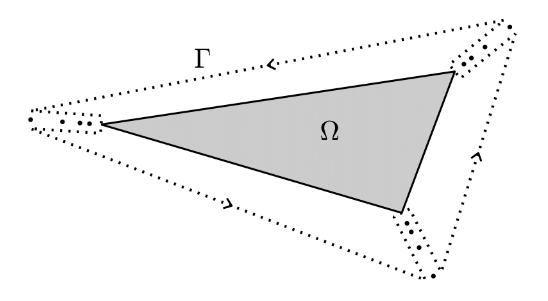
\includegraphics[scale=0.4]{./PNG/polygon_illust}\\
Split $f$ into $2m$ terms, a "Newman" part and a "Runge" part:
\begin{align*}
f=\sum_{k=1}^m f_k + \sum_{k=1}^m g_k.
\end{align*}
The Runge part can be handled by previously established results, and the Newman part can be handled by applying the first theorem to each corner.
\end{slide} %%% 12




\begin{slide} %%% 13
\large Some extensions \\

\small
Numerical experiments show that:
\begin{itemize}
	\item We can get root exponentially good approximations on non-convex domains;
	\item We're not limited to sectors and convex polygons, we can have curvy edges.
\end{itemize}
These theorems apply to an analytic function $f$, but our problem involves a harmonic $u$. 

If we assume $u$ satisfies the corner behavior needed and $\Omega$ is simply connected, then so will a $v$, where we can have an $f=u+iv$.
\end{slide} %%% 13




\begin{slide} %%% 14
\large The Algorithm 
\small
\begin{table}[h]
	\begin{tabular}{l}
		1. Define boundary $\Gamma$, corners $w_1,\ldots, w_m$, boundary function $h$,\\ tolerance $\varepsilon$.	\\
		2. For increasing values of $n$ with $\sqrt{n}$	approximately evenly spaced; \\
		\: 2a. fix $N_1=O(mn)$ poles $1/(z-z_k)$ clustered outside the corners; \\
		\: 2b. fix $N_2+1=O(n)$ monomials $1,(z-z_*),\ldots,(z-z_*)^{N_2}$\\ and set $N=N_1+N_2+1$; \\
		\: 2c. choose $M\approx 3N$ sample points on a boundary, also clustered\\ near corners; \\
		\: 2d. evaluate at sample points to obtain an $M\times N$ matrix $A$\\ and $M$-vector $b$; \\
		\: 2e. solve the least-squares problem $Ax\approx b$ for the coefficient vector $x$; \\
		\: 2f. exit loop if $||Ax-b||_\infty < \varepsilon$ or if $N$ is too large or the error is growing. \\
		3. Confirm accuracy by checking the error on a finer boundary mesh. \\
		4. Construct a function to evaluate $r(z)$ based on computed\\ coefficients $x$.
	\end{tabular}
\end{table}
\end{slide} %%% 15




\begin{slide} %%% 16
\large The code \\
\small
Code is branded "Lightning Laplace." We enter:
\begin{itemize}
	\item Corners of a polygonal-ish domain in $\mathds{C}$;
	\item boundary data in the form of a (real) function handle(s), or scalar values, corresponding to the edges.
\end{itemize}
Errors are computed by comparing the procedure with a finer sampling (so not a true error).\\
\begin{center}
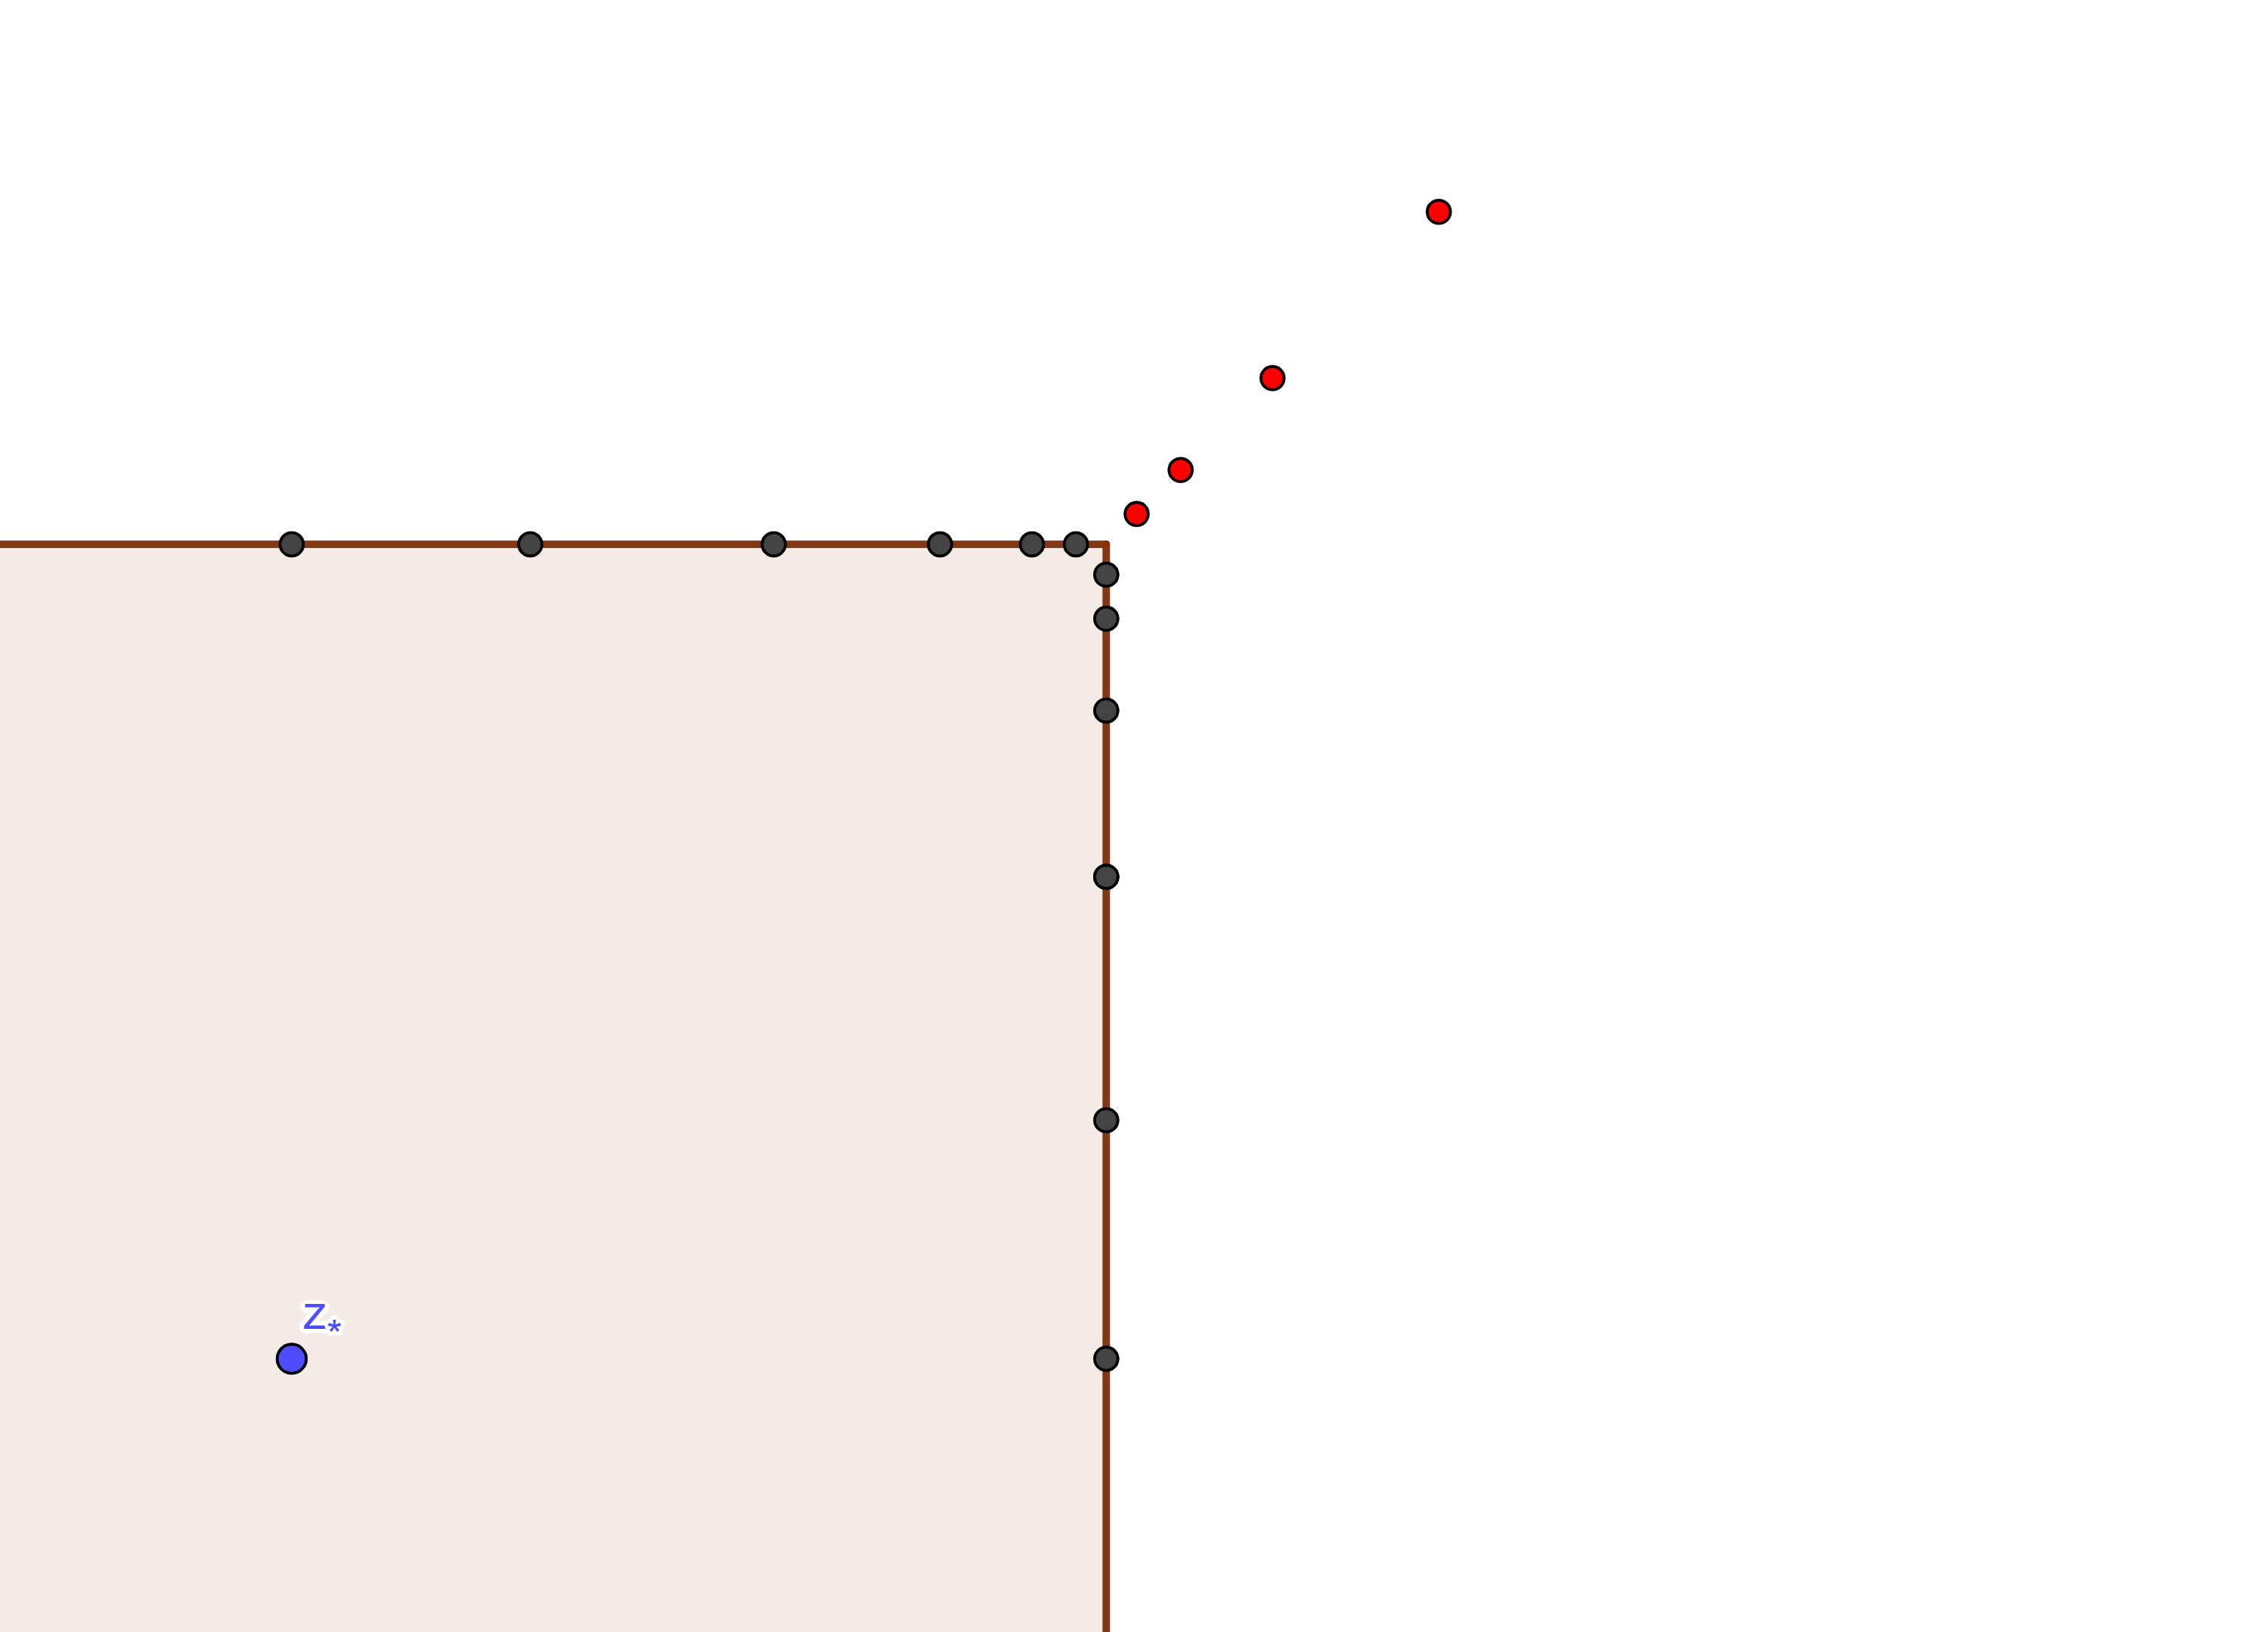
\includegraphics[scale=4]{./PNG/corner_nodes_illust}
\end{center}
\end{slide} %%% 16




\begin{slide} %%% 17

\end{slide} %%% 17



\end{document}